\section{Contribution: \'Evaluation fondée sur la recherche documentaire}

\subsection{Motivation}

\begin{frame}{Motivation}
    \textbf{Évaluation intrinsèque}
    \begin{itemize}
        \item peu fiable et pessimiste.
        \item correspondance à l'annotation sans tenir compte de leur qualité.
        %et non de la pertinence des mots-clés
    \end{itemize}
    
        %\item Étude de l'impact de l'ajout de mots-clés a des documents
    \only<2>{$\Rightarrow$ \textbf{Évaluation extrinsèque} grâce à une tâche de recherche documentaire.}
\end{frame}

\begin{frame}{Recherche documentaire}
    \begin{itemize}
        \item Retourner une liste de documents \textbf{ordonnés} par \textbf{pertinence} par rapport à une \textbf{requête}.
        \item Calcul de score grâce à des \textbf<2>{jugements de pertinence}.
    \end{itemize}
    \begin{center}
    \begin{tikzpicture}
\tikzset{
    doc/.style={rectangle, text width=0.4\linewidth, font=\footnotesize, minimum size=1cm},
    nodoc/.style={doc, fill=black!10!white,onslide={<2>fill=red!20!white}},
    okdoc/.style={doc, fill=black!10!white,onslide={<2>fill=green!20!white}}
}

\node[rectangle] at (0, 0) (titletrm) {\textbf{Requête}: Architecture of the DNA computer};
\node[below=.2cm of titletrm, xshift=-2cm, nodoc] (doc00) {An Investigation of Education of Drafting by CAD-System in the Field of Building Equipment and Machine.};
\node[below=.2cm of doc00, okdoc] (doc01) {DNA Computing and Related Fields};
\node[below=.2cm of doc01, nodoc] (doc02) {Design of a Processor Core for Massively Parallel Computers};
\node[right=.7cm of doc00, okdoc] (doc03) {A study on the computational accuracy in DNA conputation};
\node[below=.2cm of doc03, okdoc] (doc04) {Studies in Brain-Structured Supercomputers};

\node[left=.08cm of doc00] {1.};
\node[left=.08cm of doc01] {2.};
\node[left=.08cm of doc02] {3.};
\node[left=.08cm of doc03] {4.};
\node[left=.08cm of doc04] {5.};
    \end{tikzpicture}
    \end{center}
    
\end{frame}

\subsection{Cadre expérimental}

\begin{frame}{Cadre expérimental}
    \begin{block}{Systèmes de recherche d'information}
    \begin{itemize}
        \item[1.] Okapi-\bm{}~\cite{robertson_okapi_1999}
        %\item QL~\cite{ponte_language_1998} Query Likelyhood
        \item[2.] + RM3~\cite{abdul-jaleel_umass_2004}: expansion de requête
        \item \bm{} est toujours compétitive~\cite{thakur_beir_2021}
        \item Implémentations de \texttt{anserini}~\cite{yang_anserini_2017}
    \end{itemize}
    \end{block}
    \begin{block}{Collection de test}
    \begin{itemize}
        \item NTCIR-2~\cite{kando_overview_2001}: compétition de recherche ad-hoc de notices scientifiques en anglais
         \item \textbf{Mots-clés auteurs pour 98\% des documents}
        %\item Utilisation des requêtes courtes
    \end{itemize}
    \end{block}
    \vspace{-.5cm}
    \begin{table}[htbp!]
\centering
\resizebox{\textwidth}{!}{
    \begin{tabular}{rR{6.0}R{3.1}R{3.0}R{2.1}R{2.1}R{2.1}R{2.1}}
    
    %\cmidrule[1pt]{1-9}
    \toprule
            \textbf{Collection} &
            \textbf{\#Doc.} &
            \textbf{\#Dmots} &
            \textbf{\#Req.} &
            \textbf{\#Rmots} &
            \textbf{\#pert.} &
            \textbf{\#mc} &
            \textbf{\%abs} \\
    \midrule

    NTCIR-2 & 322058 & 156.8 &  49 & 11.3 & 28.8 & 4.8 & 38.1 \\
    %ACM-CR  & en & 102510 & 158.6 & 169 & 80.0 &  2.9 & 3.1 & 46.4 \\

    %\cmidrule{6-8} %\vspace{-.5em}
    %& & & & \textbf{Avg.} & 603  & 17.3  & 16.8 \\

    \bottomrule

    \end{tabular}
}
%\caption{Statistiques des collections de test NTCIR-2 et ACM-CR. La table présente le nombre de documents (\#Doc.) des collections et leur nombre moyens de mots (\#Dmots); le nombre de requête (\#Req.), leur nombre moyen de mots (\#Rmots) et le nombre moyen de document pertinent par requêtes (\#pert.); le nombre moyen de mots-clés (\#mc) par document et le ratio de mots-clés absent (\%abs) par document.}
\label{tab:collections}
\end{table}
\end{frame}

\begin{frame}{Configurations d'indexation}
    
    \alt<1>{
    1. \textbf{Titre et Résumé} \textbf{(\tr)} \phantom{la deuxième ligne av\trm}
    
    Est-ce que les mots-clés automatiques aident la recherche documentaire ?

    %{\footnotesize Les mots-clés générés remplacent-ils les mots-clés de référence ?}
    }{
    2. \textbf{Titre, Résumé et Mots-clés de référence} \textbf{(\trm)}
    %{\footnotesize Les mots-clés générés sont-ils complémentaires des mots-clés de référence ?}
    
    Est-ce que les mots-clés automatiques sont complémentaires des mots-clés auteur ?

    }
    
    \begin{columns}
    \begin{column}{.49\textwidth}
    %\vspace{.25cm}
    
    \begin{center}
    \begin{tikzpicture}[scale=.85, transform shape]
        \tikzset{rred/.style={draw=red, line width=1.6pt}}

        \pic[local bounding box=doc, rred] {docth={scale 2}};
        \node[above=.25cm of doc]{Document (T+R)};
        
        \node[rounded corners, fill=color0!40, draw=color0!80!black, align=center, text width=2.5cm, right=.7cm of doc, minimum height=2cm] (auto_prod) {\footnotesize Production automatique de mots-clés};
        \pic[local bounding box=auto_kws, onslide={<1->rred}, below=1.5cm of auto_prod] {kwsth={scale 1.5}};


        \node[below=.1cm of doc, hide, onslide=<2>show] (ref_plus) {\Huge \textbf{+}};
        %\pic[local bounding box=ref_kws, onslide={<2>rred}, below=of ref_plus] {kwsth={scale 1.5}};
        
        \begin{scope}[local bounding box=kws, scale=1.5, rred, hide, onslide=<2>show]
        \def\xdist{0-.325}
        \def\ydist{-.7-.5}
        \draw ($(ref_plus)+(\xdist,\ydist)$) rectangle +(.65,1);
        \fill[color4] ($(ref_plus)+(\xdist,\ydist)$) ++(.125,.7-.05) rectangle +(.35,.1);
        \fill[color1] ($(ref_plus)+(\xdist,\ydist)$) ++(.125,.5-.05) rectangle +(.3,.1);
        \fill[color2] ($(ref_plus)+(\xdist,\ydist)$) ++(.125,.3-.05) rectangle +(.2,.1);
        \end{scope}
        
        \node[below=.2cm of kws, text width=2cm, align=center, hide, onslide=<2>show]{Mots-clés auteur (M)};
        
        \draw[->, thick] (doc.east) -- (auto_prod.west);
        \draw[->, thick] (auto_prod.south) -- (auto_kws.north);
    \end{tikzpicture}
    \end{center}
    \end{column}
    \begin{column}{.5\textwidth}
    
    \vspace{0.5cm}
    
    \begin{block}{Ajout des 5 meilleurs mots-clés des méthodes:}
        \begin{itemize}
        \item MPRank
        \item Kea
        \item CorrRNN
        \item CopyRNN
        \end{itemize}
    \end{block}
    \end{column}
    \end{columns}
    
    %\begin{center}
        %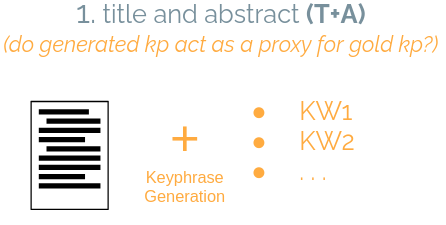
\includegraphics[align=c,width=0.4\textwidth]{figures/ri_ta.png}
        %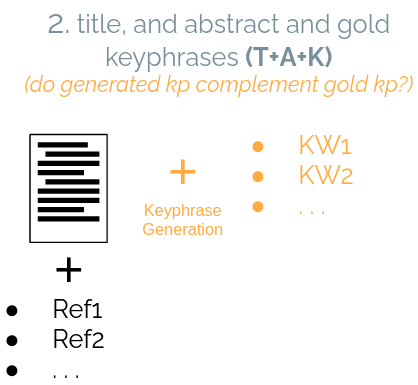
\includegraphics[align=c,width=0.4\textwidth]{figures/ri_tak.png}
    %\end{center}
\end{frame}

\subsection{Résultats}

\begin{frame}{Impact des mots-clés de référence}
    \begin{columns}
\begin{column}{.5\textwidth}
\begin{table}[!ht]
    \centering
    \setlength{\tabcolsep}{4pt}
    \resizebox{5cm}{!}{%
\begin{tabular}{l|c@{\hspace*{0mm}}r c@{\hspace*{0mm}}r|c}
    \toprule
    \textbf{Indexation} & \multicolumn{2}{c}{\textbf{BM25}} & \multicolumn{2}{c|}{\textbf{+RM3}} & F@5 \\

    \cmidrule(lr){1-6}
    \tr        & \multicolumn{2}{c}{29,6} & \multicolumn{2}{c|}{ 32,8} & -
    \alt<2->{\\
    + MPRank      & \cellcolor<3>{color1!40} 29,7 & \cellcolor<3>{color1!40} \textbf<3>{\ddiff{0,1}} & 33,0 & \ddiff{0,2} & 17,1 \\
    + Kea (KP20k) & 0,3 & \ddiff{0,7} & 33,9 & \ddiff{1,1} & 18,5\\
    \addlinespace
    + CorrRNN     & \cellcolor<3>{color2!40} \sign{31,6} & \cellcolor<3>{color2!40} \textbf<3>{\ddiff{2,1}} & \cellcolor<5>{color1!40} \bests{35,0} & \cellcolor<5>{color1!40} \ddiff{2,2} & 22,0 \\
    + CopyRNN     &  \sign{31,4} &  \ddiff{1,9} &  \sign{34,8} &  \ddiff{2,0} & 23,9 \\
    \cmidrule(lr){1-6}
    }{\\ \cmidrule(lr){1-6}}
    
    \trm & \multicolumn{2}{c}{31,9} &  \multicolumn{2}{c|}{ 35,5} & - 
    \alt<4->{\\
    + MPRank      & 32,0 & \ddiff{0,1} & 35,8 & \ddiff{0,3} & 17,1 \\
    + Kea (KP20k) & 32,1 & \ddiff{0,2} & 36,0 & \ddiff{0,5} & 18,5 \\
    \addlinespace
    + CorrRNN     & 32,4 & \ddiff{0,5} & \cellcolor<5>{color1!40} \sign{36,9} & \cellcolor<5>{color1!40} \ddiff{1,4} & 22,0 \\
    + CopyRNN     &  32,5 &  \ddiff{0,5} &   \bests{37,1} &   \ddiff{1,6} & 23,9 \\
    \bottomrule
    }{\\ \bottomrule}
    
    \end{tabular}
    }
    \caption{Scores de \map{} sur la collection NTCIR-2.}
    \label{tab:ir_results}
\end{table}
\end{column}
\begin{column}{.49\textwidth}
    \settowidth{\leftmargini}{\usebeamertemplate{itemize item}}
    \addtolength{\leftmargini}{\labelsep -.75cm}
    \begin{enumerate}
    \item<1-> Les mots-clés auteurs sont utiles !
    %\item<2-> 
    \item<3-> Les mots-clés produits par les méthodes génératives sont une \textbf<2-3>{alternative} aux mots-clés auteurs
    \item<5-> Les mots-clés de \textbf<5>{référence} et les mots-clés \textbf<5>{automatiques} sont \textbf<5>{complémentaires} !
    %\only<5>{
    %\item L'impact plus important des méthodes génératives est-il lié aux \textbf{hautes performances} de ces méthodes ou à leur \textbf{capacité générative} ?
    %}
    %\item Résultats négatifs liés à la dérive sémantique
    \end{enumerate}
\end{column}
    \end{columns}
\end{frame}

\begin{frame}{\'Evaluation de la qualité des mots-clés par une tâche applicative}
    \begin{block}{Problématique}
    \'Evaluation intrinsèque peu fiable.
    \end{block}

    Introduction d'un nouveau cadre d'\textbf{évaluation extrinsèque} fondé sur une tâche de recherche documentaire.

    \begin{block}{Conclusion}
    \begin{itemize}
        \item Mots-clés produits automatiquement sont \textbf{utiles} même \textbf{en complément} de mots-clés annotés manuellement. % (à voir par rapport a une indexation éditeur, indexeur, etc)
        \item Seules les méthodes \textbf{génératives sont assez performantes} pour impacter significativement la recherche documentaire.
        %\item Les mots-clés qui étendent le document sont les plus impactant.
    \end{itemize}
    \end{block}

\end{frame}